% Options for packages loaded elsewhere
\PassOptionsToPackage{unicode}{hyperref}
\PassOptionsToPackage{hyphens}{url}
%
\documentclass[
  ignorenonframetext,
  serif,
  professionalfont,
  usenames,
  dvipsnames,
  aspectratio = 169]{beamer}
\usepackage{pgfpages}
\setbeamertemplate{caption}[numbered]
\setbeamertemplate{caption label separator}{: }
\setbeamercolor{caption name}{fg=normal text.fg}
\beamertemplatenavigationsymbolsempty
% Prevent slide breaks in the middle of a paragraph
\widowpenalties 1 10000
\raggedbottom
\setbeamertemplate{part page}{
  \centering
  \begin{beamercolorbox}[sep=16pt,center]{part title}
    \usebeamerfont{part title}\insertpart\par
  \end{beamercolorbox}
}
\setbeamertemplate{section page}{
  \centering
  \begin{beamercolorbox}[sep=12pt,center]{part title}
    \usebeamerfont{section title}\insertsection\par
  \end{beamercolorbox}
}
\setbeamertemplate{subsection page}{
  \centering
  \begin{beamercolorbox}[sep=8pt,center]{part title}
    \usebeamerfont{subsection title}\insertsubsection\par
  \end{beamercolorbox}
}
\AtBeginPart{
  \frame{\partpage}
}
\AtBeginSection{
  \ifbibliography
  \else
    \frame{\sectionpage}
  \fi
}
\AtBeginSubsection{
  \frame{\subsectionpage}
}
\usepackage{amsmath,amssymb}
\usepackage{lmodern}
\usepackage{iftex}
\ifPDFTeX
  \usepackage[T1]{fontenc}
  \usepackage[utf8]{inputenc}
  \usepackage{textcomp} % provide euro and other symbols
\else % if luatex or xetex
  \usepackage{unicode-math}
  \defaultfontfeatures{Scale=MatchLowercase}
  \defaultfontfeatures[\rmfamily]{Ligatures=TeX,Scale=1}
\fi
% Use upquote if available, for straight quotes in verbatim environments
\IfFileExists{upquote.sty}{\usepackage{upquote}}{}
\IfFileExists{microtype.sty}{% use microtype if available
  \usepackage[]{microtype}
  \UseMicrotypeSet[protrusion]{basicmath} % disable protrusion for tt fonts
}{}
\makeatletter
\@ifundefined{KOMAClassName}{% if non-KOMA class
  \IfFileExists{parskip.sty}{%
    \usepackage{parskip}
  }{% else
    \setlength{\parindent}{0pt}
    \setlength{\parskip}{6pt plus 2pt minus 1pt}}
}{% if KOMA class
  \KOMAoptions{parskip=half}}
\makeatother
\usepackage{xcolor}
\newif\ifbibliography
\usepackage{color}
\usepackage{fancyvrb}
\newcommand{\VerbBar}{|}
\newcommand{\VERB}{\Verb[commandchars=\\\{\}]}
\DefineVerbatimEnvironment{Highlighting}{Verbatim}{commandchars=\\\{\}}
% Add ',fontsize=\small' for more characters per line
\newenvironment{Shaded}{}{}
\newcommand{\AlertTok}[1]{\textcolor[rgb]{1.00,0.00,0.00}{#1}}
\newcommand{\AnnotationTok}[1]{\textcolor[rgb]{0.00,0.50,0.00}{#1}}
\newcommand{\AttributeTok}[1]{#1}
\newcommand{\BaseNTok}[1]{#1}
\newcommand{\BuiltInTok}[1]{#1}
\newcommand{\CharTok}[1]{\textcolor[rgb]{0.00,0.50,0.50}{#1}}
\newcommand{\CommentTok}[1]{\textcolor[rgb]{0.00,0.50,0.00}{#1}}
\newcommand{\CommentVarTok}[1]{\textcolor[rgb]{0.00,0.50,0.00}{#1}}
\newcommand{\ConstantTok}[1]{#1}
\newcommand{\ControlFlowTok}[1]{\textcolor[rgb]{0.00,0.00,1.00}{#1}}
\newcommand{\DataTypeTok}[1]{#1}
\newcommand{\DecValTok}[1]{#1}
\newcommand{\DocumentationTok}[1]{\textcolor[rgb]{0.00,0.50,0.00}{#1}}
\newcommand{\ErrorTok}[1]{\textcolor[rgb]{1.00,0.00,0.00}{\textbf{#1}}}
\newcommand{\ExtensionTok}[1]{#1}
\newcommand{\FloatTok}[1]{#1}
\newcommand{\FunctionTok}[1]{#1}
\newcommand{\ImportTok}[1]{#1}
\newcommand{\InformationTok}[1]{\textcolor[rgb]{0.00,0.50,0.00}{#1}}
\newcommand{\KeywordTok}[1]{\textcolor[rgb]{0.00,0.00,1.00}{#1}}
\newcommand{\NormalTok}[1]{#1}
\newcommand{\OperatorTok}[1]{#1}
\newcommand{\OtherTok}[1]{\textcolor[rgb]{1.00,0.25,0.00}{#1}}
\newcommand{\PreprocessorTok}[1]{\textcolor[rgb]{1.00,0.25,0.00}{#1}}
\newcommand{\RegionMarkerTok}[1]{#1}
\newcommand{\SpecialCharTok}[1]{\textcolor[rgb]{0.00,0.50,0.50}{#1}}
\newcommand{\SpecialStringTok}[1]{\textcolor[rgb]{0.00,0.50,0.50}{#1}}
\newcommand{\StringTok}[1]{\textcolor[rgb]{0.00,0.50,0.50}{#1}}
\newcommand{\VariableTok}[1]{#1}
\newcommand{\VerbatimStringTok}[1]{\textcolor[rgb]{0.00,0.50,0.50}{#1}}
\newcommand{\WarningTok}[1]{\textcolor[rgb]{0.00,0.50,0.00}{\textbf{#1}}}
\usepackage{longtable,booktabs,array}
\usepackage{calc} % for calculating minipage widths
\usepackage{caption}
% Make caption package work with longtable
\makeatletter
\def\fnum@table{\tablename~\thetable}
\makeatother
\usepackage{graphicx}
\makeatletter
\def\maxwidth{\ifdim\Gin@nat@width>\linewidth\linewidth\else\Gin@nat@width\fi}
\def\maxheight{\ifdim\Gin@nat@height>\textheight\textheight\else\Gin@nat@height\fi}
\makeatother
% Scale images if necessary, so that they will not overflow the page
% margins by default, and it is still possible to overwrite the defaults
% using explicit options in \includegraphics[width, height, ...]{}
\setkeys{Gin}{width=\maxwidth,height=\maxheight,keepaspectratio}
% Set default figure placement to htbp
\makeatletter
\def\fps@figure{htbp}
\makeatother
\setlength{\emergencystretch}{3em} % prevent overfull lines
\providecommand{\tightlist}{%
  \setlength{\itemsep}{0pt}\setlength{\parskip}{0pt}}
\setcounter{secnumdepth}{-\maxdimen} % remove section numbering
% Definição do esquema de cores:
% 1. UFPR - Azul com cinza.
% 2. DEST - Roxo com cinza.
% 3. LEG - Laranjado com cinza.
\def\mycolorscheme{1}

% Caminho para a imagem de fundo com aspecto 16x9.
% \def\pathtobg{config/ufpr-fachada-baixo-1.jpg}
% \def\pathtobg{config/ufpr-fundo.jpg}
% \def\pathtobg{config/ufpr-fundo.jpg}
\def\pathtobg{./config/ufpr-fundo-16x9.jpg}

% \providecommand{\tightlist}{%
%   \setlength{\itemsep}{0pt}\setlength{\parskip}{0pt}}
% ATTENTION: Redefine o comando acima que é definido pelo template.
% \renewcommand{\tightlist}{}
\renewcommand{\tightlist}{%
  \setlength{\itemsep}{0\baselineskip}
  \setlength{\parskip}{0.25\baselineskip}
}

% Logo na capa.
\titlegraphic{
  %\vspace{-1em}
  %
\includegraphics[height=1.2cm]{config/dest-texto-2.png}\hspace{1em}
  %\includegraphics[height=1.8cm]{config/dsbd-logo-2x2.png}\hspace{1em}
  
\includegraphics[height=1.8cm]{config/ufpr-transparent-600px.png}
}
%-----------------------------------------------------------------------

% Palladio.
% \usepackage[sc]{mathpazo}
% \linespread{1.05}         % Palladio needs more leading (space between lines)
% \usepackage[T1]{fontenc}

% Kurier.
% \usepackage[light, condensed, math]{kurier}
% \usepackage[T1]{fontenc}

% Iwona.
% \usepackage[math, light, condensed]{iwona}

% \usepackage{cmbright}
% \usepackage[charter]{mathdesign}
% \usepackage{palatino}

% Roboto (with Iwona for maths).
% \usepackage[math]{iwona}
% \usepackage[sfdefault, light, condensed]{roboto}

% Source Sans Pro (with Iwona for maths).
% \usepackage[math]{iwona}
% \usepackage[default, light]{sourcesanspro}

% Lato (with Iwona for maths).
% \usepackage[math]{iwona}
% \usepackage[default]{lato}

% Fira Sans (with Iwona for maths).
\usepackage[math, light]{iwona}
\usepackage[sfdefault,light]{FiraSans} %% option 'sfdefault' activates Fira Sans as the default text font
\usepackage[T1]{fontenc}
\renewcommand*\oldstylenums[1]{{\firaoldstyle #1}}

% Font for code. ----------------------------
% \usepackage[scaled=.75]{beramono}
\usepackage{inconsolata}

% ATTENTION: needs complile with xelatex: `$ xelatex file.tex`
% \usepackage{fontspec}
% \setmonofont{M+ 1m}
% \setmonofont{M+ 1mn}
% \setmonofont{M+ 2m}

%-----------------------------------------------------------------------

% \usepackage{lmodern}
\usepackage{amssymb, amsmath}
\usepackage[makeroom]{cancel}
% \usepackage{ifxetex, ifluatex}
\usepackage{fixltx2e} % provides \textsubscript
\usepackage[utf8]{inputenc}
\usepackage[shorthands=off,main=brazil]{babel}
\usepackage{graphicx}
\usepackage{xcolor}
\usepackage{setspace}
\usepackage{comment}
\usepackage{icomma}

%-----------------------------------------------------------------------
% Algumas configurações.

\setlength{\parindent}{0pt}
\setlength{\parskip}{6pt plus 2pt minus 1pt}
\setlength{\emergencystretch}{3em}  % prevent overfull lines
% \providecommand{\tightlist}{%
%   \setlength{\itemsep}{0pt}\setlength{\parskip}{0pt}}
\setcounter{secnumdepth}{0}

% Espaço vertical para o ambiente `quote`.
\let\oldquote\quote
\let\oldendquote\endquote
\renewenvironment{quote}{%
  \vspace{1em}\oldquote}{%
  \oldendquote\vspace{1em}}

%-----------------------------------------------------------------------
% Espaçamento entre items para itemize, enumerate e description.

% % itemize.
% \let\itemopen\itemize
% \let\itemclose\enditemize
% \renewenvironment{itemize}{%
%   \itemopen\addtolength{\itemsep}{0.25\baselineskip}}{\itemclose}
%
% % enumerate.
% \let\enumopen\enumerate
% \let\enumclose\endenumerate
% \renewenvironment{enumerate}{%
%   \enumopen\addtolength{\itemsep}{0.25\baselineskip}}{\enumclose}
%
% % description.
% \let\descopen\description
% \let\descclose\enddescription
% \renewenvironment{description}{%
%   \descopen\addtolength{\itemsep}{0.25\baselineskip}}{\descclose}

%-----------------------------------------------------------------------

% \usepackage[hang]{caption}
\usepackage{caption}
\captionsetup{font=footnotesize,
  labelfont={color=mycolor1, footnotesize},
  labelsep=period}

% \providecommand{\tightlist}{%
%   \setlength{\itemsep}{0pt}\setlength{\parskip}{0pt}}

%-----------------------------------------------------------------------

\usepackage{tikz}

% \def\pathtobg{/home/walmes/Projects/templates/COMMON/ufpr-fundo.jpg}
% \def\pathtobg{/home/walmes/Projects/templates/COMMON/ufpr-fundo-16x9.jpg}
% \def\pathtobg{/home/walmes/Projects/templates/COMMON/ufpr-fachada-dir-1.jpg}
% \def\pathtobg{/home/walmes/Projects/templates/COMMON/ufpr-fachada-esq-1.jpg}
% \def\pathtobg{/home/walmes/Projects/templates/COMMON/ufpr-perto-1.jpg}
% \def\pathtobg{/home/walmes/Projects/templates/COMMON/ufpr-fachada-baixo-1.jpg}

\ifx\pathtobg\undefined
\else
  \usebackgroundtemplate{
    \tikz[overlay, remember picture]
    \node[% opacity=0.3,
          at=(current page.south east),
          anchor=south east,
          inner sep=0pt] {
            \includegraphics[height=\paperheight, width=\paperwidth]{\pathtobg}};
  }
\fi

%-----------------------------------------------------------------------
% Definições de esquema de cores.

\ifx\mycolorscheme\undefined
  % UFPR.
  % http://www.color-hex.com/color-palette/2018
  \definecolor{mycolor1}{HTML}{015c93} % Título.
  \definecolor{mycolor2}{HTML}{363435} % Texto.
  \definecolor{mycolor3}{HTML}{015c93} % Estrutura.
  \definecolor{mycolor4}{HTML}{015c93} % Links.
  \definecolor{mycolor5}{HTML}{CECAC5} % Preenchimentos.
\else
  \if\mycolorscheme1
    % UFPR.
    \definecolor{mycolor1}{HTML}{015c93} % Título.
    \definecolor{mycolor2}{HTML}{363435} % Texto.
    \definecolor{mycolor3}{HTML}{015c93} % Estrutura.
    \definecolor{mycolor4}{HTML}{015c93} % Links.
    \definecolor{mycolor5}{HTML}{CECAC5} % Preenchimentos.
  \fi
  \if\mycolorscheme2
    % DEST.
    \definecolor{mycolor1}{HTML}{2a0e72} % Título.
    \definecolor{mycolor2}{HTML}{202E35} % Texto.
    \definecolor{mycolor3}{HTML}{2a0e72} % Estrutura.
    % \definecolor{mycolor3}{HTML}{8072a3} % Estrutura.
    \definecolor{mycolor4}{HTML}{2a0e72} % Links.
    % \definecolor{mycolor4}{HTML}{bfb9d1} % Links.
    % \definecolor{mycolor5}{HTML}{AEA79F} % Preenchimentos.
    \definecolor{mycolor5}{HTML}{CECAC5} % Preenchimentos.
  \fi
  \if\mycolorscheme3
    % LEG.
    \definecolor{mycolor2}{HTML}{363435} % Texto.
    % \definecolor{mycolor1}{HTML}{ff8000} % Título.
    % \definecolor{mycolor3}{HTML}{ff8000} % Estrutura.
    % \definecolor{mycolor4}{HTML}{ff8000} % Links.
    % \definecolor{mycolor1}{HTML}{E57300} % Título.
    % \definecolor{mycolor3}{HTML}{E57300} % Estrutura.
    % \definecolor{mycolor4}{HTML}{E57300} % Links.
    \definecolor{mycolor1}{HTML}{F67014} % Título.
    \definecolor{mycolor3}{HTML}{F67014} % Estrutura.
    \definecolor{mycolor4}{HTML}{F67014} % Links.
    % \definecolor{mycolor1}{HTML}{FE5C23} % Título.
    % \definecolor{mycolor3}{HTML}{FE5C23} % Estrutura.
    % \definecolor{mycolor4}{HTML}{FE5C23} % Links.
    \definecolor{mycolor5}{HTML}{222222} % Preenchimentos.
    \definecolor{mycolor5}{HTML}{383838} % Preenchimentos.
  \fi
\fi

\hypersetup{
  colorlinks=true,
  linkcolor=mycolor4,
  urlcolor=mycolor1,
  citecolor=mycolor1
}

%-----------------------------------------------------------------------
% ATTENTION: http://www.cpt.univ-mrs.fr/~masson/latex/Beamer-appearance-cheat-sheet.pdf

\usetheme{Boadilla}
\usecolortheme{default}

% \setbeamersize{text margin left=7mm, text margin right=7mm}
% \setbeamertemplate{frametitle}[default][left, leftskip=3mm]
% \addtobeamertemplate{frametitle}{\vspace{0.5em}}{}

\setbeamertemplate{caption}[numbered]
\setbeamertemplate{section in toc}[sections numbered]
\setbeamertemplate{subsection in toc}[subsections numbered]
\setbeamertemplate{sections/subsections in toc}[ball]{}
\setbeamertemplate{sections in toc}[ball]
\setbeamercolor{section number projected}{bg=mycolor1, fg=white}
\setbeamertemplate{blocks}[rounded]
\setbeamertemplate{navigation symbols}{}
\setbeamertemplate{frametitle continuation}{\gdef\beamer@frametitle{}}
% \setbeamertemplate{frametitle}[default][center]
% \setbeamertemplate{footline}[frame number]

\setbeamertemplate{enumerate items}[default]
\setbeamertemplate{itemize items}{\scriptsize\raise1.25pt\hbox{\donotcoloroutermaths$\blacktriangleright$}}

% Blocos.
% \addtobeamertemplate{block begin}{\vskip -\bigskipamount}{}
% \addtobeamertemplate{block end}{}{\vskip -\bigskipamount}
\addtobeamertemplate{block begin}{\vspace{0.5em}}{}
\addtobeamertemplate{block end}{}{\vspace{0.5em}}


% Rodapé.
\setbeamercolor{title in head/foot}{parent=subsection in head/foot}
\setbeamercolor{author in head/foot}{bg=mycolor4, fg=white}
\setbeamercolor{date in head/foot}{parent=subsection in head/foot, fg=mycolor3}

% Cabeçalho.
\setbeamercolor{section in head/foot}{bg=mycolor2, fg=mycolor4}
\setbeamercolor{subsection in head/foot}{bg=mycolor2, fg=white}

\setbeamercolor{title}{fg=mycolor1}       % Título dos slides.
\setbeamercolor{titlelike}{fg=title}
\setbeamercolor{subtitle}{fg=mycolor2}    % Subtítulo.
\setbeamercolor{institute in head/foot}{parent=palette primary} % Instituição.
\setbeamercolor{frametitle}{fg=mycolor1}  % De quadro.
\setbeamercolor{structure}{fg=mycolor3}   % Listas e rodapé.
\setbeamercolor{item projected}{bg=mycolor2}
\setbeamercolor{block title}{bg=mycolor5, fg=mycolor2}
\setbeamercolor{normal text}{fg=mycolor2} % Texto.
\setbeamercolor{caption name}{fg=normal text.fg}
% \setbeamercolor{footlinecolor}{fg=mycolor2, bg=mycolor5}
% \setbeamercolor{section in head/foot}{fg=mycolor2, bg=mycolor5}
\setbeamercolor{author in head/foot}{fg=white, bg=mycolor1}
\setbeamercolor{section in foot}{fg=mycolor4, bg=mycolor5}
\setbeamercolor{date in foot}{fg=mycolor4, bg=mycolor5}
\setbeamercolor{block title}{fg=white, bg=mycolor1}
\setbeamercolor{block body}{fg=black, bg=white!80!gray}
\setbeamercolor{block body}{fg=black, bg=white!80!gray}

% To remove empty brackets of \institution.
\makeatletter
\setbeamertemplate{footline}{
  \leavevmode%
  \hbox{%
    \begin{beamercolorbox}[
      wd=0.3\paperwidth, ht=2.25ex, dp=1ex, right]{author in head/foot}%
      \usebeamerfont{author in head/foot}\insertshortauthor{}\hspace*{1ex}
    \end{beamercolorbox}%
    \begin{beamercolorbox}[
      wd=0.6\paperwidth, ht=2.25ex, dp=1ex, left]{section in foot}%
      \usebeamerfont{title in head/foot}\hspace*{1ex}\insertshorttitle{}
      % \usebeamerfont{title in head/foot}\hspace*{1ex}\insertframetitle{}
    \end{beamercolorbox}%
    \begin{beamercolorbox}[
      wd=0.1\paperwidth, ht=2.25ex, dp=1ex, right]{date in foot}%
      \insertframenumber{}\hspace*{2ex}
    \end{beamercolorbox}
  }%
  \vskip0pt%
}
\makeatother

%-----------------------------------------------------------------------

% \usepackage{hyphenat}
\usepackage{changepage}

% Slide para o título das seções.
\AtBeginSection[]{
  \begin{frame}
    % \vfill
    \vspace{4cm}
    % \centering
    % \begin{beamercolorbox}[sep = 8pt, center, shadow = true, rounded = true]{title}
    \begin{beamercolorbox}{title}
      \begin{columns}
        \column{0.7\linewidth}
        {\LARGE\textbf \insertsectionhead}
      \end{columns}
    \end{beamercolorbox}
    \vfill
  \end{frame}
}

%-----------------------------------------------------------------------
%---- preamble-chunk.tex -----------------------------------------------

% Knitr.

% ATTENTION: this needs `\usepackage{xcolor}'.
\definecolor{color_line}{HTML}{333333}
\definecolor{color_back}{HTML}{DDDDDD}
% \definecolor{color_back}{HTML}{FF0000}

% ATTENTION: usa o fancyvrb.
% https://ctan.math.illinois.edu/macros/latex/contrib/fancyvrb/doc/fancyvrb-doc.pdf
% R input.
\usepackage{tcolorbox}
\ifcsmacro{Highlighting}{
  % Statment if it exists. ------------------
  \DefineVerbatimEnvironment{Highlighting}{Verbatim}{
    % frame=lines,     % Linha superior e inferior.
    % framerule=0.5pt, % Espessura da linha.
    framesep=2ex,    % Distância da linha para o texto.
    % rulecolor=\color{color_line},
    % numbers=right,
    fontsize=\footnotesize, % Tamanho da fonte.
    baselinestretch=0.8,    % Espaçamento entre linhas.
    commandchars=\\\{\}}
  % Margens do ambiente `Shaded'.
  % \fvset{listparameters={\setlength{\topsep}{-1em}}}
  % \renewenvironment{Shaded}{\vspace{-1ex}}{\vspace{-2ex}}
  \renewenvironment{Shaded}{
    \vspace{2pt}
    \begin{tcolorbox}[
      boxrule=0pt,      % Espessura do contorno.
      colframe=gray!10, % Cor do contorno.
      colback=gray!10,  % Cor de fundo da caixa.
      arc=1em,          % Raio para contornos arredondados.
      sharp corners,
      boxsep=0.5em,     % Margem interna.
      left=3pt, right=3pt, top=3pt, bottom=3pt, % Margens internas.
      grow to left by=0mm,
      grow to right by=6pt,
      ]
    }{
    \end{tcolorbox}
    \vspace{-3pt}
    }
  }{
  % Statment if it not exists. --------------
}

% R output e todo `verbatim'.
\makeatletter
\def\verbatim@font{\linespread{0.8}\ttfamily\footnotesize}
%\makeatother

% Cor de fundo e margens do `verbatim'.
\let\oldv\verbatim
\let\oldendv\endverbatim

\def\verbatim{%
  \par\setbox0\vbox\bgroup % Abre grupo.
  %\vspace{-5px}            % Reduz margem superior.
  \oldv                    % Chama abertura do verbatim.
}
\def\endverbatim{%
  \oldendv                 % Chama encerramento do verbatim.
  %\vspace{0cm}           % Controla margem inferior.
  \egroup%\fboxsep5px      % Fecha grupo.
  \noindent{{\usebox0}}\par
}

%-----------------------------------------------------------------------
%---- preamble-commands.tex --------------------------------------------

% Para fazer texto em duas colunas.
\newcommand{\mytwocolumns}[4]{
  % #1: Line width fraction for the left column , e.g. 0.5.
  % #2: Line width fraction for the right column.
  % #3: Content for the left column.
  % #4: Content for the right column.
  \begin{columns}[c]
    \begin{column}{#1\linewidth} %----------- left.
      #3
    \end{column} %--------------------------- left.
    \begin{column}{#2\linewidth} %----------- right.
      #4
    \end{column} %--------------------------- right.
  \end{columns}
}

%-----------------------------------------------------------------------
% Para fazer duas colunas no Rmd.

% Center vertical align.
\def\beginAHalfColumn{\begin{minipage}{0.49\textwidth}}%
\def\beginAlmostHalfColumn{\begin{minipage}{0.45\textwidth}}%
\def\beginAQuarterColumn{\begin{minipage}{0.23\textwidth}}%
\def\beginThreeQuartersColumn{\begin{minipage}{0.72\textwidth}}%
\def\beginAThirdColumn{\begin{minipage}{0.31\textwidth}}%
\def\beginTwoThirdsColumn{\begin{minipage}{0.64\textwidth}}%
\def\endColumns{\end{minipage}}%

% Top vertical align.
\def\beginAHalfColumnT{\begin{minipage}[t]{0.49\textwidth}}%
\def\beginAlmostHalfColumnT{\begin{minipage}[t]{0.45\textwidth}}%
\def\beginAQuarterColumnT{\begin{minipage}[t]{0.23\textwidth}}%
\def\beginThreeQuartersColumnT{\begin{minipage}[t]{0.72\textwidth}}%
\def\beginAThirdColumnT{\begin{minipage}[t]{0.31\textwidth}}%
\def\beginTwoThirdsColumnT{\begin{minipage}[t]{0.64\textwidth}}%

%---------------------------------------------------------------------
% Ambientes para frases como e sem imagem.

\newcommand{\myquote}[3]{
  % #1: caminho para a imagem.
  % #2: a frase/quotation.
  % #3: o autor.
  \begin{center}
    \begin{minipage}[c]{0.19\linewidth}
      \begin{center}
        \includegraphics[height=2.5cm]{#1}
      \end{center}
    \end{minipage}
    \begin{minipage}[c]{0.7\linewidth}
      \begin{flushright}
        \textit{#2}
        \vspace{1ex}

        -- #3
      \end{flushright}
    \end{minipage}
  \end{center}
}

\newcommand{\myphrase}[2]{
  % #1: a frase/quotation.
  % #2: o autor.
  \begin{center}
    \begin{minipage}[c]{0.19\linewidth}
    \end{minipage}
    \begin{minipage}[c]{0.7\linewidth}
      \begin{flushright}
        \textit{#1}
        \vspace{1ex}

        -- #2
      \end{flushright}
    \end{minipage}
  \end{center}
}

%-----------------------------------------------------------------------
% Comandos para texto em destaque.

% \newcommand{\hi}[1]{%
%   \textcolor{ubuntu_orange}{#1}\xspace
% }

\usepackage{xspace}

% URLs com letra miuda.
\newcommand{\myurl}[1]{%
  {\tiny \url{#1}}\xspace
}

% Botões.
\newcommand{\btn}[1]{%
  \beamergotobutton{#1}\xspace
}

% Texto grande centralizado.
\newcommand{\centertitle}[1]{%
  \begin{center}
    {\LARGE \bfseries \hi{#1}}
  \end{center}
}

%-----------------------------------------------------------------------
\ifLuaTeX
  \usepackage{selnolig}  % disable illegal ligatures
\fi
\IfFileExists{bookmark.sty}{\usepackage{bookmark}}{\usepackage{hyperref}}
\IfFileExists{xurl.sty}{\usepackage{xurl}}{} % add URL line breaks if available
\urlstyle{same} % disable monospaced font for URLs
\hypersetup{
  pdfauthor={Prof.~Me. Lineu Alberto Cavazani de Freitas},
  hidelinks,
  pdfcreator={LaTeX via pandoc}}

\title{\textbf{Primeiros passos com R}}
\subtitle{R no RStudio, primeiros passos, R como calculadora, variáveis
e funções básicas}
\author{Prof.~Me. Lineu Alberto Cavazani de Freitas}
\date{}
\institute{Métodos Estatísticos em Pesquisa Científica\\
Apoio computacional em linguagem R\\
\strut \\
Departamento de Estatística\\
Laboratório de Estatística e Geoinformação}

\begin{document}
\frame{\titlepage}

\begin{frame}{Introdução}
\protect\hypertarget{introduuxe7uxe3o}{}
\begin{itemize}
\item
  O R é uma \textbf{linguagem de programação}.
\item
  Uma linguagem de programação é a forma que nós nos comunicamos com o
  computador.
\item
  Escrevemos um código R para que o computador entenda e execute a
  tarefa de interesse.
\item
  O R trabalha com a ideia de interface de linha de comando (command
  line interface).
\item
  Precisamos escrever os códigos para que a linguagem passe para o
  computador executar.
\end{itemize}
\end{frame}

\begin{frame}{Introdução}
\protect\hypertarget{introduuxe7uxe3o-1}{}
\beginAHalfColumn

\begin{itemize}
\tightlist
\item
  Atenção:

  \begin{itemize}
  \tightlist
  \item
    O R é a \textbf{linguagem}.
  \item
    O RStudio é a \textbf{interface}.
  \item
    Quem faz o trabalho (manda a solicitação para que o computador
    execute) é o R!
  \end{itemize}
\end{itemize}

\endColumns
\beginAHalfColumn

\begin{figure}

{\centering 
\includegraphics[width=0.6\linewidth]{./img/atencao} 

}

\caption{Extraído de \href{https://cdn.pixabay.com/photo/2013/04/01/10/57/exclamation-mark-98739_1280.png}{pixabay.com.}}\label{fig:unnamed-chunk-2}
\end{figure}

\endColumns
\end{frame}

\begin{frame}{Introdução}
\protect\hypertarget{introduuxe7uxe3o-2}{}
\begin{itemize}
\tightlist
\item
  Geralmente, trabalhando em R escrevemos o código, executamos,
  avaliamos o resultado e seguimos acrescentando as instruções até obter
  o resultado esperado.

  \begin{itemize}
  \tightlist
  \item
    Modo \textbf{REPL}: Read, Eval, Print and Loop
  \end{itemize}
\item
  Outra forma de trabalhar é escrever toda a sequência de código e
  executá-la de uma única vez.

  \begin{itemize}
  \tightlist
  \item
    Esta ideia é útil para ambientes de produção nos quais não há
    supervisão.
  \item
    Chamado de modo \textbf{Batch}.
  \end{itemize}
\end{itemize}
\end{frame}

\hypertarget{abrindo-o-rstudio}{%
\section{Abrindo o RStudio}\label{abrindo-o-rstudio}}

\begin{frame}{Abrindo o RStudio}
\protect\hypertarget{abrindo-o-rstudio-1}{}
\beginAHalfColumn

\begin{itemize}
\item
  O RStudio como IDE tem o papel de facilitar o trabalho em R.
\item
  Portanto, ao abrir o RStudio, tudo que você precisa deve estar à
  mostra e com fácil acesso.
\item
  Ao abrir o RStudio você verá uma estrutura organizada em paineis.
\end{itemize}

\endColumns
\beginAHalfColumn

\begin{figure}

{\centering 
\includegraphics[width=0.6\linewidth]{./img/rstudiologo} 

}

\caption{Logo do RStudio.}\label{fig:unnamed-chunk-3}
\end{figure}

\endColumns
\end{frame}

\begin{frame}{Abrindo o RStudio}
\protect\hypertarget{abrindo-o-rstudio-2}{}
\begin{figure}

{\centering 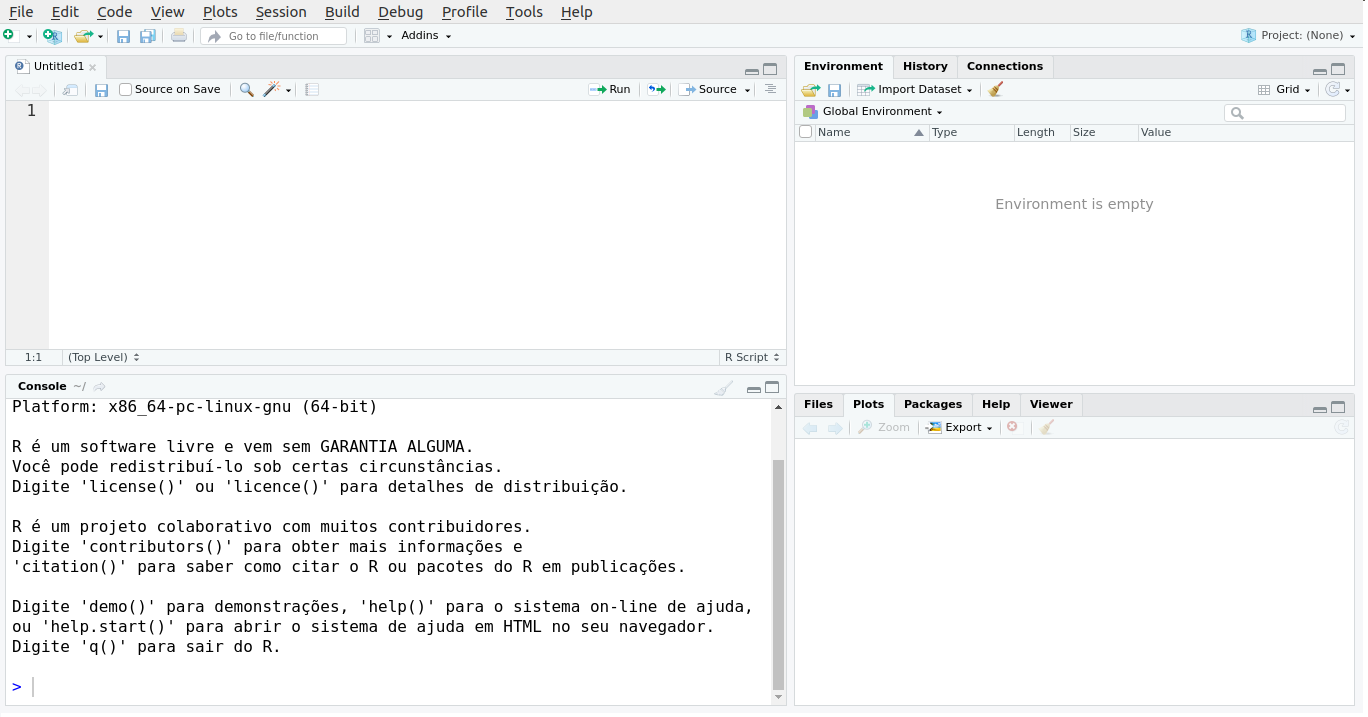
\includegraphics[width=0.85\linewidth]{./img/rstudio} 

}

\caption{Tela inicial do RStudio.}\label{fig:unnamed-chunk-4}
\end{figure}
\end{frame}

\begin{frame}[fragile]{Paineis}
\protect\hypertarget{paineis}{}
\begin{itemize}
\item
  No \textbf{canto superior esquerdo} é onde digitamos o código R que
  será executado: o \textbf{editor}.

  \begin{itemize}
  \tightlist
  \item
    Se o R está recém instalado ou a sessão é nova, crie um arquivo .R
    clicando em
    \texttt{File\ \textgreater{}\ New\ File\ \textgreater{}\ R} ou use
    as teclas de atalho \texttt{Ctrl\ +\ Shift\ +\ N}.
  \end{itemize}
\item
  No \textbf{canto inferior esquerdo} é onde o terminal R está, é ali
  onde o código é interpretado e executado: o \textbf{console}.
\item
  No canto superior direito são mostradas informações do ambiente de
  trabalho, histórico, conexões, etc.
\item
  No canto inferior direito são apresentados os arquivos da pasta de
  trabalho, gráficos, pacotes, documentação etc.
\end{itemize}
\end{frame}

\begin{frame}{Editor}
\protect\hypertarget{editor}{}
\begin{figure}

{\centering 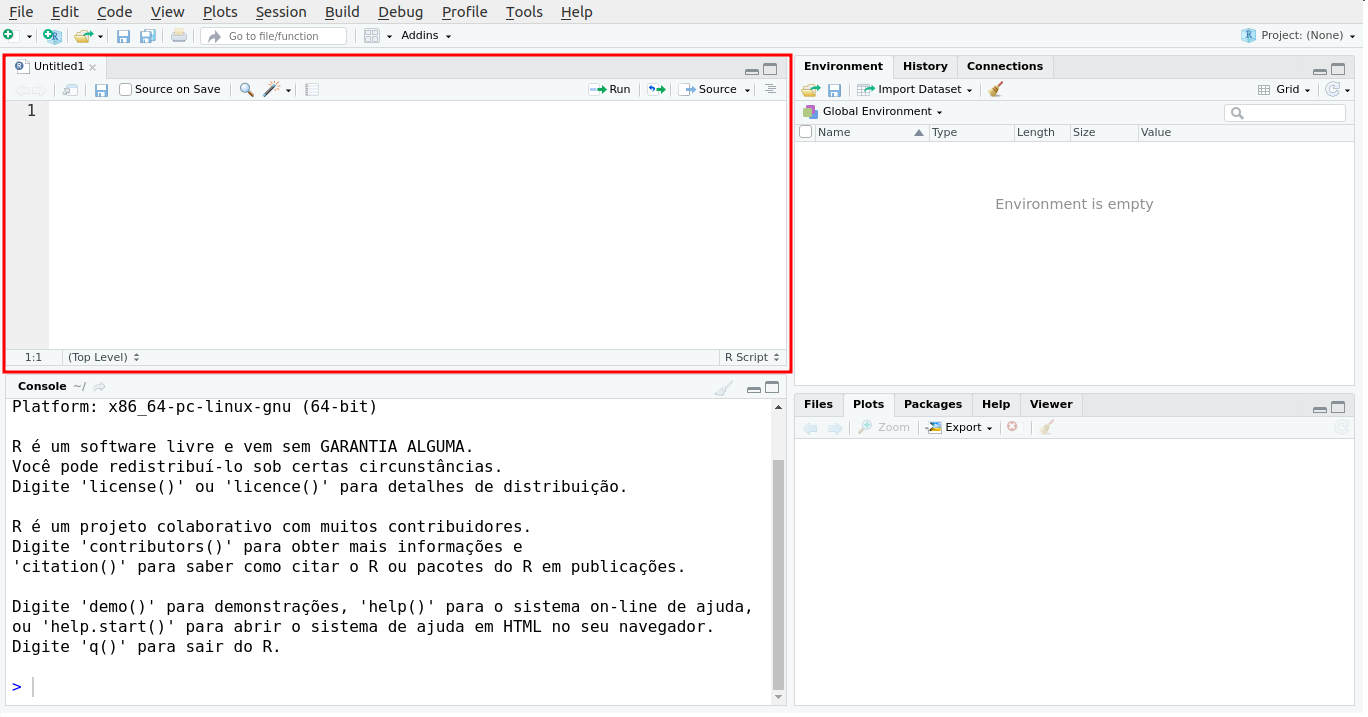
\includegraphics[width=0.85\linewidth]{./img/editor} 

}

\caption{Tela inicial do RStudio. Foco no editor.}\label{fig:unnamed-chunk-5}
\end{figure}
\end{frame}

\begin{frame}{Console}
\protect\hypertarget{console}{}
\begin{figure}

{\centering 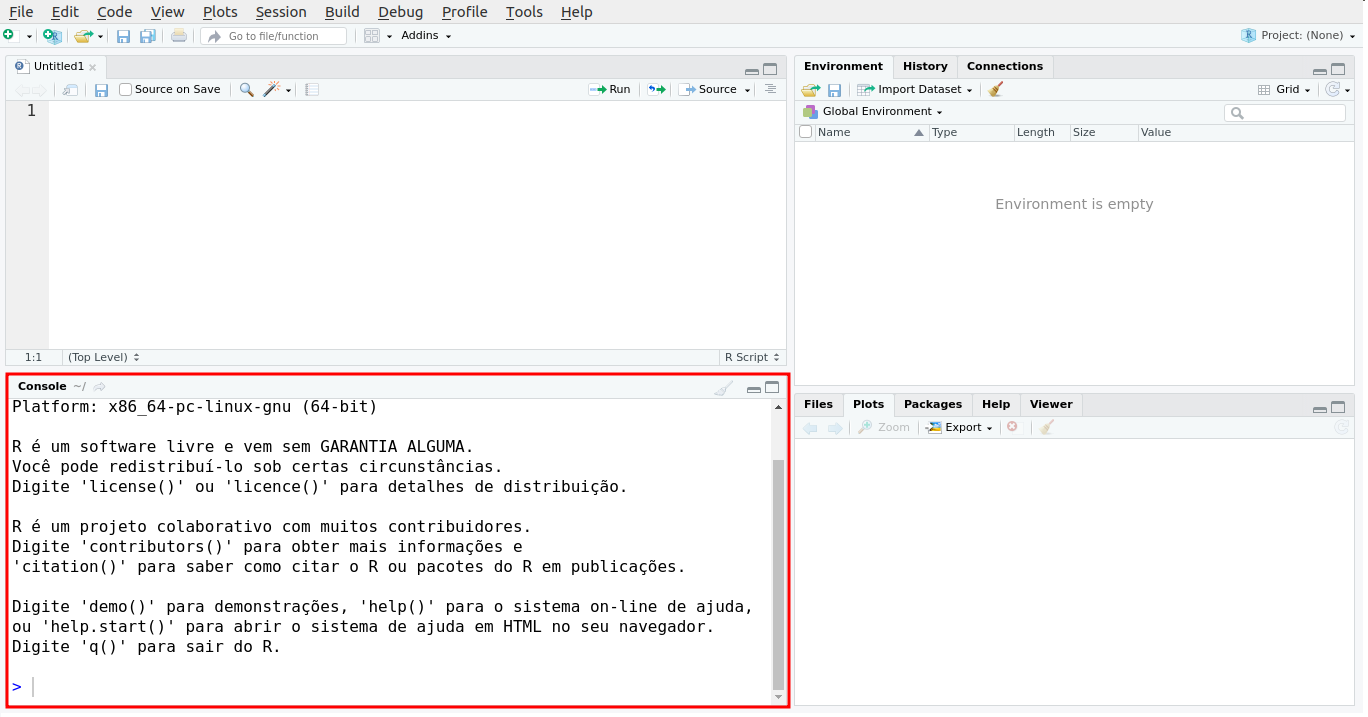
\includegraphics[width=0.85\linewidth]{./img/console} 

}

\caption{Tela inicial do RStudio. Foco no console.}\label{fig:unnamed-chunk-6}
\end{figure}
\end{frame}

\begin{frame}{Ambiente, histórico, conexões}
\protect\hypertarget{ambiente-histuxf3rico-conexuxf5es}{}
\begin{figure}

{\centering 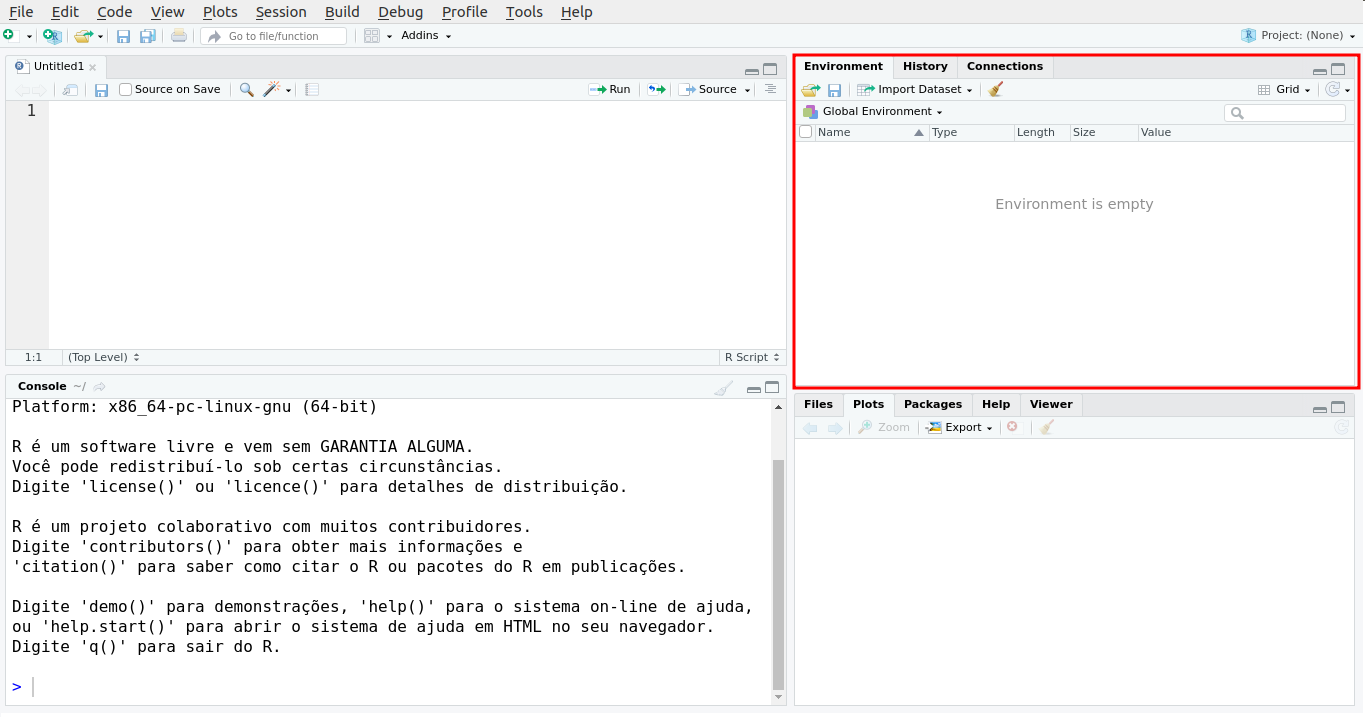
\includegraphics[width=0.85\linewidth]{./img/env} 

}

\caption{Tela inicial do RStudio. Foco no ambiente, histórico e conexões.}\label{fig:unnamed-chunk-7}
\end{figure}
\end{frame}

\begin{frame}{Arquivos, gráficos, pacotes e documentação}
\protect\hypertarget{arquivos-gruxe1ficos-pacotes-e-documentauxe7uxe3o}{}
\begin{figure}

{\centering 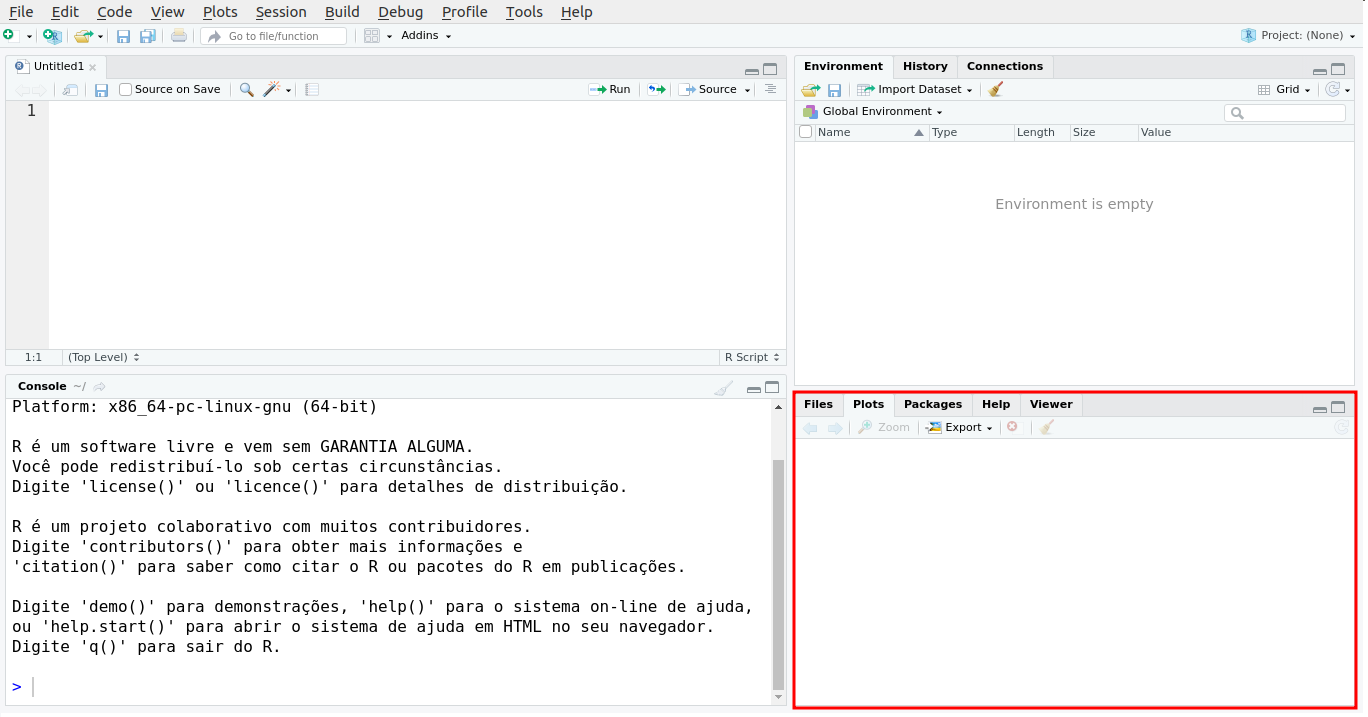
\includegraphics[width=0.85\linewidth]{./img/files} 

}

\caption{Tela inicial do RStudio. Foco nos arquivos, pacotes e documentação.}\label{fig:unnamed-chunk-8}
\end{figure}
\end{frame}

\begin{frame}[fragile]{Principais elementos}
\protect\hypertarget{principais-elementos}{}
Em resumo:

\begin{itemize}
\tightlist
\item
  \textbf{Editor}: onde escrevemos os códigos.
\item
  \textbf{Console}: onde os resultados são printados.
\item
  \textbf{Environment}: mostra todos os objetos criados.
\item
  \textbf{History}: mostra todos os códigos executados.
\item
  \textbf{Files}: mostra os arquivos no diretório atual.
\item
  \textbf{Plots}: mostra os outputs de códigos que geram gráficos.
\item
  \textbf{Packages}: mostra os pacotes instalados.
\item
  \textbf{Help}: mostra a documentação de funções e pacotes.
\end{itemize}

\textbf{Dica}: Para obter todos os atalhos da interface digite pressione
\texttt{ALT+SHIFT+K}.
\end{frame}

\begin{frame}[fragile]{Customizando o RStudio}
\protect\hypertarget{customizando-o-rstudio}{}
\beginAHalfColumn

\begin{itemize}
\item
  O RStudio permite customizar os elementos.
\item
  Experimente acessar
  \texttt{Tools\ \textgreater{}\ Global\ Options\ \textgreater{}\ Appearance}
  para trocar temas, ordem dos paineis, tamanho da fonte, etc.
\item
  Deixe o RStudio confortável para você.
\end{itemize}

\endColumns
\beginAHalfColumn

\begin{figure}

{\centering 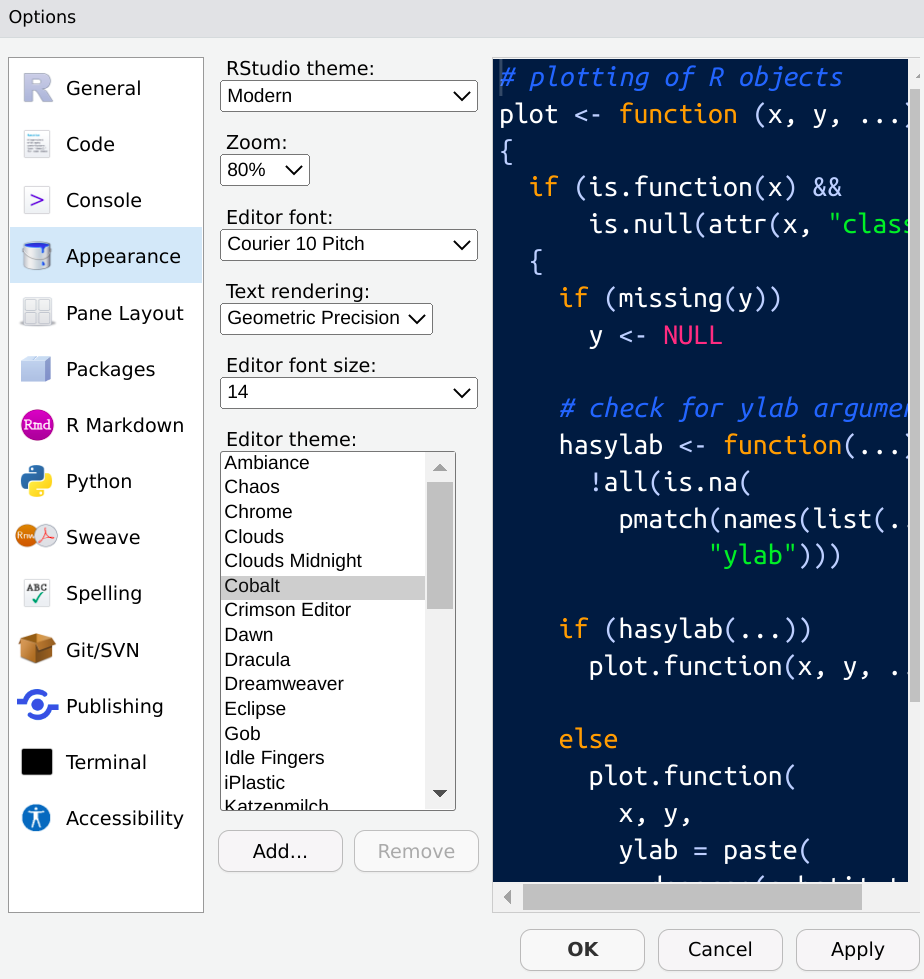
\includegraphics[width=0.85\linewidth]{./img/aparencia} 

}

\caption{Tela inicial do RStudio.}\label{fig:unnamed-chunk-9}
\end{figure}

\endColumns
\end{frame}

\hypertarget{trabalhando-com-r-no-rstudio}{%
\section{Trabalhando com R no
RStudio}\label{trabalhando-com-r-no-rstudio}}

\begin{frame}[fragile]{Primeiros passos}
\protect\hypertarget{primeiros-passos}{}
\begin{enumerate}
\item
  Crie uma pasta em algum lugar do seu computador para trabalhar.
\item
  Abra o RStudio e defina o diretório de trabalho.

  \begin{itemize}
  \tightlist
  \item
    O diretório de trabalho é a pasta do R onde estamos trabalhando.
  \item
    \texttt{Session\ \textgreater{}\ Set\ Working\ Directory\ \textgreater{}\ Choose\ Directory...}
    ou \texttt{CTRL\ +\ SHIFT\ +\ H}.

    \begin{itemize}
    \tightlist
    \item
      Ambas as opções darão a possibilidade de escolher a pasta de
      interesse no computador onde manteremos nossos arquivos.
    \end{itemize}
  \end{itemize}
\end{enumerate}
\end{frame}

\begin{frame}[fragile]{Primeiros passos}
\protect\hypertarget{primeiros-passos-1}{}
\begin{enumerate}
\setcounter{enumi}{2}
\tightlist
\item
  Crie um arquivo com extensão .R.

  \begin{itemize}
  \tightlist
  \item
    \texttt{File\ \textgreater{}\ New\ File\ \textgreater{}\ R\ script}.
  \item
    \texttt{CTRL\ +\ SHIFT\ +\ N}.
  \end{itemize}
\item
  Salve seu script.

  \begin{itemize}
  \tightlist
  \item
    Esta etapa funciona como qualquer arquivo do computador.
  \item
    \texttt{File\ \textgreater{}\ Save} ou \texttt{CTRL\ +\ S}.
  \item
    De um nome para seu arquivo.

    \begin{itemize}
    \tightlist
    \item
      Opte por nomes curtos, intuitivos e evite espaços, acentos e
      caracteres.
    \end{itemize}
  \end{itemize}
\end{enumerate}

Agora estamos prontos para trabalhar!
\end{frame}

\begin{frame}[fragile]{Instruções e comentários}
\protect\hypertarget{instruuxe7uxf5es-e-comentuxe1rios}{}
\begin{itemize}
\item
  Uma \textbf{instrução} é um código a ser executado.
\item
  Um \textbf{comentário} é algo que escrevemos no script mas que não
  temos interesse que seja executado.
\item
  Comentários podem e devem ser usados para \textbf{documentar} o
  código.
\item
  Tudo que vier após \texttt{\#} é um comentário e não será executado
  pela linguagem.
\end{itemize}
\end{frame}

\begin{frame}[fragile]{Executando}
\protect\hypertarget{executando}{}
\begin{itemize}
\item
  Para executar uma instrução no RStudio basta ir até a linha de
  interesse e teclar \texttt{CTRL\ +\ ENTER}.
\item
  O código é interpretado, executado e o resultado é mostrado na tela.
\item
  Uma recomendação para scripts mais organizados é não ultrapassar
  \(72\) ou \(80\) caracteres por linha.
\item
  Outra recomendação diz respeito à indentação ou alinhamento do código.

  \begin{itemize}
  \tightlist
  \item
    Use \texttt{CTRL+i} no RStudio para indentar automaticamente.
  \end{itemize}
\end{itemize}
\end{frame}

\hypertarget{r-como-calculadora}{%
\section{R como calculadora}\label{r-como-calculadora}}

\begin{frame}{R como calculadora}
\protect\hypertarget{r-como-calculadora-1}{}
\begin{itemize}
\item
  O R pode ser usado como uma poderosa \textbf{calculadora científica}.
\item
  Os operadores seguem uma hierarquia, ou seja, uma ordem de
  precedência.

  \begin{itemize}
  \tightlist
  \item
    Inicialmente são efetuadas as operações entre parênteses seguindo a
    ordem: exponenciação, multiplicação/divisão e por fim
    adição/subtração.
  \end{itemize}
\item
  Para utilizar os operadores no R basta digitar os valores e a operação
  diretamente no console (caso queira ver somente o resultado) ou no
  editor (caso deseje salvar o código no arquivo .R).
\end{itemize}
\end{frame}

\begin{frame}[fragile]{Operações aritméticas básicas}
\protect\hypertarget{operauxe7uxf5es-aritmuxe9ticas-buxe1sicas}{}
\beginAThirdColumn

\begin{Shaded}
\begin{Highlighting}[]
\CommentTok{\# Soma}
\DecValTok{1} \SpecialCharTok{+} \DecValTok{1} 
\end{Highlighting}
\end{Shaded}

\begin{verbatim}
## [1] 2
\end{verbatim}

\begin{Shaded}
\begin{Highlighting}[]
\CommentTok{\# Subtração}
\DecValTok{1} \SpecialCharTok{{-}} \DecValTok{1} 
\end{Highlighting}
\end{Shaded}

\begin{verbatim}
## [1] 0
\end{verbatim}

\begin{Shaded}
\begin{Highlighting}[]
\CommentTok{\# Multiplicação}
\DecValTok{2} \SpecialCharTok{*} \DecValTok{2} 
\end{Highlighting}
\end{Shaded}

\begin{verbatim}
## [1] 4
\end{verbatim}

\endColumns
\beginAThirdColumn

\begin{Shaded}
\begin{Highlighting}[]
\CommentTok{\# Divisão}
\DecValTok{4}\SpecialCharTok{/}\DecValTok{2} 
\end{Highlighting}
\end{Shaded}

\begin{verbatim}
## [1] 2
\end{verbatim}

\begin{Shaded}
\begin{Highlighting}[]
\CommentTok{\# Potenciação}
\DecValTok{5}\SpecialCharTok{\^{}}\DecValTok{2} 
\end{Highlighting}
\end{Shaded}

\begin{verbatim}
## [1] 25
\end{verbatim}

\begin{Shaded}
\begin{Highlighting}[]
\CommentTok{\# Radiciação}
\DecValTok{2}\SpecialCharTok{\^{}}\NormalTok{(}\DecValTok{1}\SpecialCharTok{/}\DecValTok{3}\NormalTok{) }
\end{Highlighting}
\end{Shaded}

\begin{verbatim}
## [1] 1.259921
\end{verbatim}

\endColumns
\beginAThirdColumn

\begin{Shaded}
\begin{Highlighting}[]
\CommentTok{\# Resto}
\DecValTok{10} \SpecialCharTok{\%\%} \DecValTok{3}
\end{Highlighting}
\end{Shaded}

\begin{verbatim}
## [1] 1
\end{verbatim}

\begin{Shaded}
\begin{Highlighting}[]
\CommentTok{\# Parte inteira}
\DecValTok{10} \SpecialCharTok{\%/\%} \DecValTok{3} 
\end{Highlighting}
\end{Shaded}

\begin{verbatim}
## [1] 3
\end{verbatim}

\endColumns
\end{frame}

\begin{frame}[fragile]{Funções trigonométricas}
\protect\hypertarget{funuxe7uxf5es-trigonomuxe9tricas}{}
\beginAHalfColumn

\begin{Shaded}
\begin{Highlighting}[]
\CommentTok{\# Seno}
\FunctionTok{sin}\NormalTok{(}\DecValTok{0}\NormalTok{) }
\end{Highlighting}
\end{Shaded}

\begin{verbatim}
## [1] 0
\end{verbatim}

\begin{Shaded}
\begin{Highlighting}[]
\CommentTok{\# Cosseno}
\FunctionTok{cos}\NormalTok{(}\DecValTok{0}\NormalTok{) }
\end{Highlighting}
\end{Shaded}

\begin{verbatim}
## [1] 1
\end{verbatim}

\begin{Shaded}
\begin{Highlighting}[]
\CommentTok{\# Tangente}
\FunctionTok{tan}\NormalTok{(}\DecValTok{0}\NormalTok{) }
\end{Highlighting}
\end{Shaded}

\begin{verbatim}
## [1] 0
\end{verbatim}

\endColumns
\beginAHalfColumn

\begin{Shaded}
\begin{Highlighting}[]
\CommentTok{\# Arco seno}
\FunctionTok{asin}\NormalTok{(}\DecValTok{0}\NormalTok{)}
\end{Highlighting}
\end{Shaded}

\begin{verbatim}
## [1] 0
\end{verbatim}

\begin{Shaded}
\begin{Highlighting}[]
\CommentTok{\# Arco cosseno}
\FunctionTok{acos}\NormalTok{(}\DecValTok{1}\NormalTok{) }
\end{Highlighting}
\end{Shaded}

\begin{verbatim}
## [1] 0
\end{verbatim}

\begin{Shaded}
\begin{Highlighting}[]
\CommentTok{\# Arco tangente}
\FunctionTok{atan}\NormalTok{(}\DecValTok{0}\NormalTok{) }
\end{Highlighting}
\end{Shaded}

\begin{verbatim}
## [1] 0
\end{verbatim}

\endColumns
\end{frame}

\begin{frame}[fragile]{Funções matemáticas especiais}
\protect\hypertarget{funuxe7uxf5es-matemuxe1ticas-especiais}{}
\beginAThirdColumn

\begin{Shaded}
\begin{Highlighting}[]
\CommentTok{\# Exponencial base e}
\FunctionTok{exp}\NormalTok{(}\DecValTok{1}\NormalTok{)}
\end{Highlighting}
\end{Shaded}

\begin{verbatim}
## [1] 2.718282
\end{verbatim}

\begin{Shaded}
\begin{Highlighting}[]
\CommentTok{\# Raiz quadrada}
\FunctionTok{sqrt}\NormalTok{(}\DecValTok{4}\NormalTok{) }
\end{Highlighting}
\end{Shaded}

\begin{verbatim}
## [1] 2
\end{verbatim}

\begin{Shaded}
\begin{Highlighting}[]
\CommentTok{\# Log neperiano}
\FunctionTok{log}\NormalTok{(}\DecValTok{10}\NormalTok{) }
\end{Highlighting}
\end{Shaded}

\begin{verbatim}
## [1] 2.302585
\end{verbatim}

\endColumns
\beginAThirdColumn

\begin{Shaded}
\begin{Highlighting}[]
\CommentTok{\# Log qualquer base}
\FunctionTok{log}\NormalTok{(}\DecValTok{10}\NormalTok{, }\AttributeTok{base =} \DecValTok{5}\NormalTok{) }
\end{Highlighting}
\end{Shaded}

\begin{verbatim}
## [1] 1.430677
\end{verbatim}

\begin{Shaded}
\begin{Highlighting}[]
\CommentTok{\# Fatorial}
\FunctionTok{factorial}\NormalTok{(}\DecValTok{4}\NormalTok{)}
\end{Highlighting}
\end{Shaded}

\begin{verbatim}
## [1] 24
\end{verbatim}

\begin{Shaded}
\begin{Highlighting}[]
\CommentTok{\# Valor absoluto}
\FunctionTok{abs}\NormalTok{(}\SpecialCharTok{{-}}\DecValTok{1}\NormalTok{) }
\end{Highlighting}
\end{Shaded}

\begin{verbatim}
## [1] 1
\end{verbatim}

\endColumns
\beginAThirdColumn

\begin{Shaded}
\begin{Highlighting}[]
\CommentTok{\# Arredondamento para cima}
\FunctionTok{ceiling}\NormalTok{(}\FloatTok{1.2}\NormalTok{)}
\end{Highlighting}
\end{Shaded}

\begin{verbatim}
## [1] 2
\end{verbatim}

\begin{Shaded}
\begin{Highlighting}[]
\CommentTok{\# Arredondamento para baixo}
\FunctionTok{floor}\NormalTok{(}\FloatTok{1.2}\NormalTok{)}
\end{Highlighting}
\end{Shaded}

\begin{verbatim}
## [1] 1
\end{verbatim}

\begin{Shaded}
\begin{Highlighting}[]
\CommentTok{\# Arredondamento}
\FunctionTok{round}\NormalTok{(}\FloatTok{1.2}\NormalTok{, }\AttributeTok{digits =} \DecValTok{0}\NormalTok{)  }
\end{Highlighting}
\end{Shaded}

\begin{verbatim}
## [1] 1
\end{verbatim}

\endColumns
\end{frame}

\begin{frame}[fragile]{Operadores lógicos}
\protect\hypertarget{operadores-luxf3gicos}{}
\beginAThirdColumn

\begin{Shaded}
\begin{Highlighting}[]
\CommentTok{\# São iguais?}
\DecValTok{1} \SpecialCharTok{==} \DecValTok{1} 
\end{Highlighting}
\end{Shaded}

\begin{verbatim}
## [1] TRUE
\end{verbatim}

\begin{Shaded}
\begin{Highlighting}[]
\CommentTok{\# São iguais?}
\DecValTok{1} \SpecialCharTok{==} \DecValTok{2} 
\end{Highlighting}
\end{Shaded}

\begin{verbatim}
## [1] FALSE
\end{verbatim}

\begin{Shaded}
\begin{Highlighting}[]
\CommentTok{\# São diferentes?}
\DecValTok{2} \SpecialCharTok{!=} \DecValTok{2} 
\end{Highlighting}
\end{Shaded}

\begin{verbatim}
## [1] FALSE
\end{verbatim}

\endColumns
\beginAThirdColumn

\begin{Shaded}
\begin{Highlighting}[]
\CommentTok{\# São diferentes?}
\DecValTok{1} \SpecialCharTok{!=} \DecValTok{2} 
\end{Highlighting}
\end{Shaded}

\begin{verbatim}
## [1] TRUE
\end{verbatim}

\begin{Shaded}
\begin{Highlighting}[]
\CommentTok{\# 2 é menor ou igual a 1?}
\DecValTok{2} \SpecialCharTok{\textless{}=} \DecValTok{1}
\end{Highlighting}
\end{Shaded}

\begin{verbatim}
## [1] FALSE
\end{verbatim}

\begin{Shaded}
\begin{Highlighting}[]
\CommentTok{\# 2 é maior ou igual a 1?}
\DecValTok{2} \SpecialCharTok{\textgreater{}=} \DecValTok{1} 
\end{Highlighting}
\end{Shaded}

\begin{verbatim}
## [1] TRUE
\end{verbatim}

\endColumns
\beginAThirdColumn

\begin{Shaded}
\begin{Highlighting}[]
\CommentTok{\# 2 é maior do que 1?}
\DecValTok{2} \SpecialCharTok{\textgreater{}} \DecValTok{1} 
\end{Highlighting}
\end{Shaded}

\begin{verbatim}
## [1] TRUE
\end{verbatim}

\begin{Shaded}
\begin{Highlighting}[]
\CommentTok{\# 2 é menor do que 1?}
\DecValTok{2} \SpecialCharTok{\textless{}} \DecValTok{1} 
\end{Highlighting}
\end{Shaded}

\begin{verbatim}
## [1] FALSE
\end{verbatim}

\endColumns
\end{frame}

\begin{frame}[fragile]{E, OU e NÃO}
\protect\hypertarget{e-ou-e-nuxe3o}{}
\beginAHalfColumn

\begin{itemize}
\item
  Combinação de resultados lógicos.
\item
  1 é menor que 5 \textbf{E} 2 é maior ou igual a 3?
\end{itemize}

\begin{Shaded}
\begin{Highlighting}[]
\NormalTok{(}\DecValTok{1} \SpecialCharTok{\textless{}} \DecValTok{5}\NormalTok{) }\SpecialCharTok{\&}\NormalTok{ (}\DecValTok{2} \SpecialCharTok{\textgreater{}=} \DecValTok{3}\NormalTok{)}
\end{Highlighting}
\end{Shaded}

\begin{verbatim}
## [1] FALSE
\end{verbatim}

\begin{itemize}
\tightlist
\item
  1 é menor que 5 \textbf{OU} 2 é maior ou igual a 3?
\end{itemize}

\begin{Shaded}
\begin{Highlighting}[]
\NormalTok{(}\DecValTok{1} \SpecialCharTok{\textless{}} \DecValTok{5}\NormalTok{) }\SpecialCharTok{|}\NormalTok{ (}\DecValTok{2} \SpecialCharTok{\textgreater{}=} \DecValTok{3}\NormalTok{)}
\end{Highlighting}
\end{Shaded}

\begin{verbatim}
## [1] TRUE
\end{verbatim}

\endColumns
\beginAHalfColumn

\begin{itemize}
\tightlist
\item
  2 é menor que 5? Inverta a resposta lógica.
\end{itemize}

\begin{Shaded}
\begin{Highlighting}[]
\SpecialCharTok{!}\NormalTok{(}\DecValTok{2} \SpecialCharTok{\textless{}} \DecValTok{5}\NormalTok{)}
\end{Highlighting}
\end{Shaded}

\begin{verbatim}
## [1] FALSE
\end{verbatim}

\endColumns
\end{frame}

\begin{frame}[fragile]{Valores especiais}
\protect\hypertarget{valores-especiais}{}
\beginAThirdColumn

\begin{itemize}
\tightlist
\item
  NA: valores ausentes.
\item
  NULL: objetos vazios.
\item
  Inf e -Inf: infinitos.
\item
  NaN: indeterminações.
\end{itemize}

\endColumns
\beginAThirdColumn

\begin{Shaded}
\begin{Highlighting}[]
\DecValTok{1} \SpecialCharTok{+} \ConstantTok{NA}
\end{Highlighting}
\end{Shaded}

\begin{verbatim}
## [1] NA
\end{verbatim}

\begin{Shaded}
\begin{Highlighting}[]
\DecValTok{1} \SpecialCharTok{+} \ConstantTok{NULL}
\end{Highlighting}
\end{Shaded}

\begin{verbatim}
## numeric(0)
\end{verbatim}

\endColumns
\beginAThirdColumn

\begin{Shaded}
\begin{Highlighting}[]
\DecValTok{1}\SpecialCharTok{/}\DecValTok{0}
\end{Highlighting}
\end{Shaded}

\begin{verbatim}
## [1] Inf
\end{verbatim}

\begin{Shaded}
\begin{Highlighting}[]
\DecValTok{0}\SpecialCharTok{/}\DecValTok{0}
\end{Highlighting}
\end{Shaded}

\begin{verbatim}
## [1] NaN
\end{verbatim}

\endColumns
\end{frame}

\hypertarget{variuxe1veis}{%
\section{Variáveis}\label{variuxe1veis}}

\begin{frame}[fragile]{Variáveis}
\protect\hypertarget{variuxe1veis-1}{}
\begin{itemize}
\item
  No R podemos usar \textbf{objetos} para atribuir valores que serão
  usados recorrentemente.
\item
  Por exemplo, suponha que estamos trabalhando com o valor \(10\) e que
  este valor será usado várias e várias vezes no código.
\item
  Para poupar algum trabalho, podemos atribuir este valor a um objeto.
  Por exemplo, \texttt{x}:
\end{itemize}

\begin{Shaded}
\begin{Highlighting}[]
\NormalTok{x }\OtherTok{\textless{}{-}} \DecValTok{10}
\end{Highlighting}
\end{Shaded}
\end{frame}

\begin{frame}[fragile]{Variáveis}
\protect\hypertarget{variuxe1veis-2}{}
\begin{itemize}
\item
  Usamos o operador de atribuição \texttt{\textless{}-} (lemos RECEBE)
  para atribuir o valor \(10\) à variável \texttt{x}.
\item
  O sinal de igual (\texttt{=}) também pode ser usado, mas o
  \texttt{\textless{}-} é mais comum e recomendado.
\item
  Note que ao fazer uma atribuição o resultado não é printado no
  terminal.
\item
  Para que o resultado seja printado, digite o nome da variável em uma
  nova linha e execute.
\end{itemize}
\end{frame}

\begin{frame}[fragile]{Variáveis}
\protect\hypertarget{variuxe1veis-3}{}
\begin{itemize}
\item
  Ao fazer uma atribuição, criamos um objeto na nossa área de trabalho.
\item
  Para listar os objetos criados na área de trabalho usamos a função
  \texttt{ls()}.
\item
  Se repetirmos o código de atribuição com outro valor, vamos o
  sobrescrever. Portanto, cuidado!
\item
  Quando há a necessidade de apagar um objeto da área de trabalho usamos
  a função \texttt{rm()}.
\end{itemize}
\end{frame}

\begin{frame}[fragile]{Variáveis}
\protect\hypertarget{variuxe1veis-4}{}
\beginAHalfColumn

\begin{Shaded}
\begin{Highlighting}[]
\CommentTok{\# Atribui o valor 10 à variável x}
\NormalTok{x }\OtherTok{\textless{}{-}} \DecValTok{10}

\CommentTok{\# Printa o valor de x}
\NormalTok{x}
\end{Highlighting}
\end{Shaded}

\begin{verbatim}
## [1] 10
\end{verbatim}

\begin{Shaded}
\begin{Highlighting}[]
\CommentTok{\# Lista as variáveis}
\FunctionTok{ls}\NormalTok{()}
\end{Highlighting}
\end{Shaded}

\begin{verbatim}
## [1] "format_field" "thm"          "x"
\end{verbatim}

\endColumns
\beginAHalfColumn

\begin{Shaded}
\begin{Highlighting}[]
\CommentTok{\# Remove a variável x}
\FunctionTok{rm}\NormalTok{(x)}

\CommentTok{\# Lista as variáveis}
\FunctionTok{ls}\NormalTok{()}
\end{Highlighting}
\end{Shaded}

\begin{verbatim}
## [1] "format_field" "thm"
\end{verbatim}

\endColumns
\end{frame}

\hypertarget{funuxe7uxf5es-buxe1sicas}{%
\section{Funções básicas}\label{funuxe7uxf5es-buxe1sicas}}

\begin{frame}{Funções básicas}
\protect\hypertarget{funuxe7uxf5es-buxe1sicas-1}{}
\begin{itemize}
\item
  Além dos objetos, \textbf{funções} são um elemento importante em R.
\item
  Na prática funções também são objetos.
\item
  O R já vem com diversas funções básicas.
\item
  Algumas já vimos nos operadores matemáticos.
\end{itemize}
\end{frame}

\begin{frame}{Funções básicas}
\protect\hypertarget{funuxe7uxf5es-buxe1sicas-2}{}
\begin{longtable}[]{@{}
  >{\centering\arraybackslash}p{(\columnwidth - 2\tabcolsep) * \real{0.2933}}
  >{\centering\arraybackslash}p{(\columnwidth - 2\tabcolsep) * \real{0.7067}}@{}}
\toprule()
\begin{minipage}[b]{\linewidth}\centering
Função
\end{minipage} & \begin{minipage}[b]{\linewidth}\centering
Tarefa
\end{minipage} \\
\midrule()
\endhead
c() & Cria um Vetor \\
setwd() & Muda o Diretório de Trabalho Atual \\
getwd() & Mostra o Diretório de Trabalho \\
dir() & Lista os Arquivos do Diretório de Trabalho Atual \\
sessionInfo() & Mostra algumas informações da sessão \\
install.packages() & Instala um pacote \\
library() & Carrega um pacote \\
require() & Carrega um pacote \\
example() & Mostra exemplos de alguma função \\
print() & Imprime o resultado de uma variável \\
q() & Fecha a Sessão \\
objects() & Exibe objetos criados \\
str() & Mostra a estrutura de um objeto \\
\bottomrule()
\end{longtable}
\end{frame}

\hypertarget{funuxe7uxf5es-de-ajuda}{%
\section{Funções de ajuda}\label{funuxe7uxf5es-de-ajuda}}

\begin{frame}{Funções de ajuda}
\protect\hypertarget{funuxe7uxf5es-de-ajuda-1}{}
\begin{itemize}
\item
  Algo ótimo de se trabalhar em R é a \textbf{documentação interna}.
\item
  Em R cada função e objeto tem a sua própria documentação.
\item
  Em alguns casos, para pacotes que fazem algumas análises especificas,
  temos tutoriais que são chamados de \textbf{vinhetas} (vignettes).
\item
  Existem funções que auxiliam no acesso à documentação.
\end{itemize}
\end{frame}

\begin{frame}[fragile]{Funções de ajuda}
\protect\hypertarget{funuxe7uxf5es-de-ajuda-2}{}
\begin{itemize}
\item
  Para acessar a documentação específica de uma função ou objeto podemos
  usar as funções \texttt{?} ou \texttt{help()}.
\item
  A documentação aparecerá no painel no canto inferior direito do
  RStudio.
\item
  Suponha que você não saiba exatamente o nome da função ou objeto para
  o qual você quer consultar a documentação.
\item
  Neste caso, você pode procurar por funções e objetos por meio de algum
  termo de busca com a função \texttt{help.search()}.
\end{itemize}
\end{frame}

\begin{frame}[fragile]{Funções de ajuda}
\protect\hypertarget{funuxe7uxf5es-de-ajuda-3}{}
\begin{itemize}
\item
  Uma outra forma de obter ajuda é usar a função \texttt{apropos()}.
\item
  Ela vai procurar por objetos no caminho de procura que batem com o
  termo que você está procurando.
\item
  Já as vignettes estão associadas a pacotes específicos.
\item
  Podemos consultar todos os vignettes disponíveis dentro de um pacote
  com a função \texttt{browseVignettes()}.
\item
  O R abrirá uma nova janela em seu browser onde mostrará os títulos dos
  vignettes disponíveis para o pacote solicitado.
\item
  Outra possibilidade é a função \texttt{RSiteSearch()} que fará uma
  busca mais geral procurando pelo termo no site oficial do R
  (r-project.org).
\end{itemize}
\end{frame}

\begin{frame}[fragile]{Funções de ajuda}
\protect\hypertarget{funuxe7uxf5es-de-ajuda-4}{}
\begin{Shaded}
\begin{Highlighting}[]
\CommentTok{\# Solicita a documentação interna do pacote base}
\NormalTok{?base}
\FunctionTok{help}\NormalTok{(base)}

\CommentTok{\# Busca pelo termo \textquotesingle{}linear models\textquotesingle{}}
\FunctionTok{help.search}\NormalTok{(}\StringTok{"linear models"}\NormalTok{)}

\CommentTok{\# Busca funções e objetos pelo nome parcial}
\FunctionTok{apropos}\NormalTok{(}\StringTok{"plot"}\NormalTok{)}

\CommentTok{\# Busca vinhetas}
\FunctionTok{browseVignettes}\NormalTok{(}\StringTok{"grid"}\NormalTok{)}

\CommentTok{\# Busca um termo no site do R}
\FunctionTok{RSiteSearch}\NormalTok{(}\StringTok{"plot"}\NormalTok{)}
\end{Highlighting}
\end{Shaded}
\end{frame}

\begin{frame}{Campos da documentação}
\protect\hypertarget{campos-da-documentauxe7uxe3o}{}
Os campos e seus respectivos conteúdos são os seguintes:

\begin{itemize}
\tightlist
\item
  \textbf{Cabeçalho}: indica o pacote.
\item
  \textbf{Título}: título da função.
\item
  \textbf{Description}: descrição do que o objeto é/faz.
\item
  \textbf{Usage}: como usar ou fazer a chamada.
\item
  \textbf{Arguments}: quais os argumentos formais da função.
\item
  \textbf{Value}: o que a função retorna.
\item
  \textbf{Details}: detalhes adicionais de implementação.
\item
  \textbf{Note}: notas adicionais sobre uso e afins.
\item
  \textbf{See Also}: referências para documentação relacionada.
\item
  \textbf{References}: referências bibliográficas.
\item
  \textbf{Authors}: autores da função.
\item
  \textbf{Examples}: exemplos de uso.
\end{itemize}
\end{frame}

\begin{frame}{Funções de ajuda}
\protect\hypertarget{funuxe7uxf5es-de-ajuda-5}{}
\begin{itemize}
\item
  O R possui uma documentação completa e com diversas opções para
  acesso.
\item
  Não se preocupe em decorar comandos.
\item
  Quando necessário, saiba onde consultar!
\item
  Com o tempo e experiência acabamos nos habituando com diversos
  comandos.
\item
  Mas crie o hábito de acessar documentação interna e também pesquisar
  na web ``como fazer\ldots{} no R''.
\item
  Pesquisas em inglês aumentam a chance de êxito.
\end{itemize}
\end{frame}

\hypertarget{arquivos-da-linguagem}{%
\section{Arquivos da linguagem}\label{arquivos-da-linguagem}}

\begin{frame}{Arquivos da linguagem}
\protect\hypertarget{arquivos-da-linguagem-1}{}
\begin{itemize}
\item
  Ao usar uma sessão R existem alguns arquivos que são gerados.
\item
  Mencionaremos 2 que costumam ser bastante úteis: \textbf{.Rhistory} e
  \textbf{.RData}.
\item
  \textbf{.Rhistory}: salva todos os comandos executados em uma sessão
  R. Ele é cirado por default ao abrir uma sessão e caso exista um
  .Rhistory no atual diretório de trabalho ele é carregado
  automaticamente.
\item
  \textbf{.RData}: durante uma sessão podemos criar muitos objetos.
  Estes objetos podem ser importantes, de difícil obtenção ou até mesmo
  custosos em termos de tempo e tamanho. O .RData serve para salvar os
  objetos de uma sessão. Ao abrir uma nova sessão e carregar o .RData,
  todos os objetos estarão lá e não precisarão ser gerados novamente.
\end{itemize}
\end{frame}

\begin{frame}[fragile]{Arquivos da linguagem}
\protect\hypertarget{arquivos-da-linguagem-2}{}
\begin{Shaded}
\begin{Highlighting}[]
\CommentTok{\# Salvando o histórico de comandos}
\FunctionTok{savehistory}\NormalTok{(}\AttributeTok{file =} \StringTok{"historico.Rhistory"}\NormalTok{)}

\CommentTok{\# Salvando todas as variáveis criadas na sessão}
\FunctionTok{save.image}\NormalTok{(}\AttributeTok{file =} \StringTok{"variaveis.RData"}\NormalTok{)}
\end{Highlighting}
\end{Shaded}
\end{frame}

\hypertarget{pacotes}{%
\section{Pacotes}\label{pacotes}}

\begin{frame}{Pacotes}
\protect\hypertarget{pacotes-1}{}
\begin{itemize}
\item
  No R a principal forma de contribuição da comunidade é por meio de
  pacotes.
\item
  Os pacotes são coleções de funções e/ou conjuntos de dados organizados
  e documentados.
\item
  Um pacote R pode conter código R e também de outras linguagens como C,
  Fortran e C++.
\item
  Alguns pacotes podem depender de bibliotecas do seu sistema
  operacional, as chamadas libs.
\end{itemize}
\end{frame}

\begin{frame}[fragile]{Pacotes}
\protect\hypertarget{pacotes-2}{}
\begin{itemize}
\item
  Existem repositórios oficiais como o CRAN, Biocondutor e MRAN.
\item
  O CRAN o mais famoso e usual.
\item
  A instalação do pacote é feita usando a função
  \texttt{install.packages()}.
\item
  Outra possibilidade é obter arquivos compactados (em geral .tar.gz) e
  fazer uma instalação manual.
\item
  Outra fonte de pacotes são os repositórios de próprios desenvolvedores
  em plataformas de versionamento de código como o Git, GitHub, GitLab,
  entre outros.
\end{itemize}
\end{frame}

\begin{frame}[fragile]{Pacotes}
\protect\hypertarget{pacotes-3}{}
\begin{itemize}
\tightlist
\item
  Por exemplo, podemos instalar o pacote \texttt{ggplot2} pelo próprio
  R.
\end{itemize}

\begin{Shaded}
\begin{Highlighting}[]
\CommentTok{\# instalando o pacote ggplot2 do CRAN}
\FunctionTok{install.packages}\NormalTok{(}\StringTok{"ggplot2"}\NormalTok{)}
\end{Highlighting}
\end{Shaded}

\begin{itemize}
\tightlist
\item
  Para as funções de um pacote poderem ser usadas precisamos carregar o
  pacote com a função \texttt{library()}.
\end{itemize}

\begin{Shaded}
\begin{Highlighting}[]
\FunctionTok{library}\NormalTok{(ggplot2)}
\end{Highlighting}
\end{Shaded}

\begin{itemize}
\tightlist
\item
  Podemos analisar o conteúdo e a documentação de um pacote.
\end{itemize}

\begin{Shaded}
\begin{Highlighting}[]
\FunctionTok{ls}\NormalTok{(}\StringTok{"package:ggplot2"}\NormalTok{) }\CommentTok{\# conteúdo do pacote}
\FunctionTok{help}\NormalTok{(}\AttributeTok{package =} \StringTok{"ggplot2"}\NormalTok{) }\CommentTok{\# documentação do pacote}
\end{Highlighting}
\end{Shaded}
\end{frame}

\end{document}
